\documentclass[main.tex]{subfiles}

\begin{document}

\chapter{%
\texorpdfstring{\boldmath{\(\ket{0}\rightarrow\ket{1}\)}}{0 -> 1} state evolution
}
In this simulation, the optimization was run to realise the state evolution \(\ket{0}\rightarrow\ket{1}\).
The pulse shape should be close to the ideal solution of a \(\pi\)-pulse: a gaussian pulse which performs a bit flip on a qubit.
Therefore it is a suitable goal to test the method and package.


\section{Simulation Setup}
In this section the Hamiltonian and the optimization parameters will be presented.

\subsection{Hamiltonian}
The anharmonic resonator (qubit) in~\Cref{eq:resonator-hamiltonian} was chosen as it is a simple model for a physical qubit.
As stated earlier such a system will be referred to as a qubit even though it has more than two energy levels.
To induce transitions between the states of the qubit, control pulse terms were added to~\Cref{eq:resonator-hamiltonian}, resulting in
\begin{equation}
    \Ham = \omega_{q} \au\ad + \frac{K_q}{2} (\au)^2\ad^2 + \Omega(t)\ex^{-i\omega_{q}t}\ad + \Omega^*(t)\ex^{i\omega_{q}t}\au,
    \label{eq:system-hamiltonian}
\end{equation}
where \( \Omega(t) \) is the complex amplitude of the control pulse.
Looking at the Hamiltonian above, it can be argued that it can be written in the form in \Cref{eq:optimal-control-hamiltonian}, which is needed by \krotov{}, with \( u_0(t) = \Omega(t)\ex^{i\omega_{q}t} \) and \( u_1(t) = \Omega^*(t)\ex^{-i\omega_{q}t} \).
However, there are two problems that need to be adressed.
Firstly, the oscillating factors require an unnecessarily fine time discretization of the pulses.
Secondly, the Krotov package expects real-valued pulse amplitudes \( \qty{u_i(t)} \) as inputs.
The first problem was avoided by transforming the Hamiltonian into the interaction picture with respect to \(\omega_{q} \au\ad \), also known as the rotating frame.
That is the Hamiltonian is transformed with
\begin{equation}
    \hat{U}\Ham\hat{U}^\dagger + i\dv{\hat{U}}{t}\hat{U}^\dagger,
\end{equation}
where \( \hat{U} = \ex^{-i\omega_{q} \au\ad t} \) which results in
%Now \Cref{eq:system-hamiltonian} transforms\footnote{Full derivation is shown in \Cref{sec:appendix-interaction-picture}} into
\begin{equation}
    \Ham \rightarrow~ \frac{K_q}{2}(\au)^2\ad^2 + \Omega(t)\ad + \Omega^*(t)\au.
    \label{eq:krotov-hamiltonian-rotating}
\end{equation}
Now the pulse amplitudes \( u_0(t) = \Omega(t) \) and \( u_1(t) = \Omega^*(t) \), i.e.\ the envelope of the physical control pulse which varies significantly slower than the actual pulse.
The second problem was easily fixed with a rearrangment of the terms
\[ \Omega(t)\ad + \Omega^*(t)\au = \bigg[\text{Re}\qty[\Omega(t)]+i\text{Im}\qty[\Omega(t)]\bigg]\ad + \bigg[\text{Re}\qty[\Omega(t)]-i\text{Im}\qty[\Omega(t)]\bigg]\au = \]
\[ = \text{Re}\qty[\Omega(t)]\qty(\ad + \au) + \text{Im}\qty[\Omega(t)]i\qty(\ad - \au). \]
For intuition, \( \qty(\ad + \au) \) and \( i\qty(\ad - \au) \) correspond to rotations around the Bloch sphere\footnote{A quick explanation of how the Bloch sphere is used for visualization is given in \Cref{sec:bloch-sphere}.} along the x-axis and y-axis respectively. 
Thus the final Hamiltonian became
\begin{equation}
    \Ham = \underbrace{K_q/2(\au)^2\ad^2}_{\Ham_d} + \underbrace{\text{Re}\qty[\Omega(t)]}_{u_0(t)}\underbrace{(\ad + \au)}_{\Ham_0} + \underbrace{\text{Im}\qty[\Omega(t)]}_{u_1(t)}\underbrace{i(\ad - \au)}_{\Ham_1} .
    \label{eq:system-hamiltonian-rotating}
\end{equation}

The parameters of the qubit were chosen to model real superconducting qubits with \( K_q = 2\pi\times\SI{297}{\mega\hertz} \) (and \( \omega_{q} = 2\pi\times\SI{6.2815}{\giga\hertz} \)).
The system Hamiltonian in \Cref{eq:system-hamiltonian-rotating} was simulated with a truncated Hilbert space size conveniently chosen to be \( N_q = 3 \).
A smaller truncated Hilbert space, and consequently smaller matrices, requires less computations but could possibly yield a poor approximation of the Hamiltonian.
Thus the solutions of the optimization were analysed with this in mind.

\subsection{Optimization Setup}
As the long-term goal is to use this method in physical systems some constraints were added.
To simulate the constraints of physical arbitrary waveform generators (AWG) a maximum sample rate of \SI{4}{\giga\samples\per\second} was chosen.
Recall that the physcal pulses oscillate at \( \omega_{q} = \SI{6.2815}{\giga\hertz} \), a rate which \SI{4}{\giga\samples\per\second} can impossibly resolve.
Although AWGs with higher sample rates than \SI{4}{\giga\samples\per\second} exist, they are expensive.
However, rotating frame transformation permits the use of a relatively low rate AWG to generate the pulse envelopes \( \Omega(t) \) and a high rate tone generator to create a carrier signal at \( \omega_{q} \), with these signals later combined in a mixer.
Further, due to the noise sensitivity of superconducting systems an amplitude constraint is needed to keep the system cool enough.
To set a realistic maximum amplitude \( A_m \) some derivation was required.
First the maximum amplitude was chosen with the assumption that a gaussian pulse
\begin{equation}
    g(t) = \frac{\pi/2}{\sigma\sqrt{2\pi}} \ex^{-\frac{1}{2}\qty(\frac{t}{\sigma})^2}
\end{equation}
with \( \sigma = \ns{3} \) can physically realise a \(\pi\)-rotation \( \ket{0} \rightarrow \ket{1} \) in a planar transmon qubit.
The problem with gaussian pulses however is that they do not go to zero at the edges.
To fix this \krotov{} provides a function for generating Blackman pulses.
A Blackman pulse with a total length of \(6\sigma\) is a good approximation of a Gaussian pulse, with the added benefit of going to zero at the edges.
However, due to the approximation, the integral of the Blackman pulse will not exactly be equal to the integral of the corresponding gaussian pulse, which is needed to realise the \(\pi\)-rotation.
This can be fixed by using a prefactor \(C\) which can be calculated by solving
\begin{equation}
    C \int_0^{6\sigma}\frac{1}{\sqrt{2\pi}\sigma} B(t) = \int_0^{6\sigma}g(t-3\sigma)\id t
\end{equation}
where \(B(t)\) is the Blackman pulse.
This is now used to determine the maximum amplitude
\begin{equation}
    A(\sigma) = \frac{C}{\text{max}(\sigma,3)\sqrt{2\pi}}
\end{equation}
with \(A_m = A(\sigma = 3)\). 
This amplitude constraint is enforced by calling a function after every iteration which limits all pulse shape values \(|\Omega| < A_m\).
Conveniently, the Blackman pulse was also used as the initial guess pulse with \(u_0(t) = A(T/6)B(t),\, u_1(t)=0\).

Another constraint was added so that the edges of the pulses were always zero.
This was done with a switch-on/switch-off of \ns{2}.
This ramp shape is half a Blackman pulse and is provided by \krotov{}'s \texttt{flattop} function.

For the \(\ket{0}\rightarrow\ket{1}\) state evolution, pulse shapes were optimized with varying lengths from \SI{4.25}{\nano\second} to \SI{30}{\nano\second} with convergence criteria \(F>0.99999\) or \(\Delta F < \num{e-07}\).
The step size was chosen as \(\lambda = \frac{1}{\frac{1}{2}A_{m}}\).
The reason for optimizing for various pulse lengths was that faster pulse changes gives a broader support in the frequency spectrum which can ultimately induce transitions in other levels.
Therefore the optimization needs to find a solution which circumvents this problem.

\section{Results}
\begin{figure}[H]
    \centering
    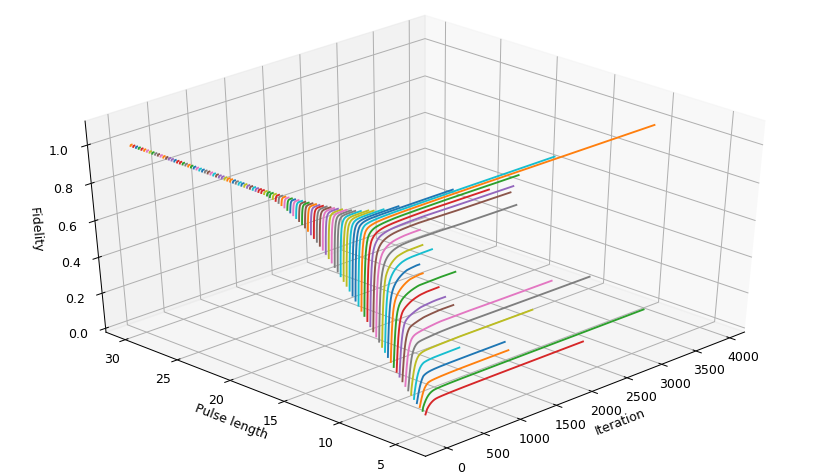
\includegraphics[width=\linewidth]{figs/3d-optim-ge.png}
    \caption{Fidelity during optimizations for every pulse length (ns). The different colors help distinguish the lines.}\label{fig:3d-optim-ge}
\end{figure}

In \Cref{fig:3d-optim-ge} the fidelity during all optimizations (with pulse lengths from \ns{4.25} to \ns{30}) are plotted.
The ``starting fidelity'' is the fidelity which is obtained with the guess pulses while the ``optimized fidelity'' is the fiedlity obtained with the optimized pulses.
For pulse lengths longer than \SI{15}{\nano\second} the fidelity starts at values close to the goal (\(F>0.9\)) and the number of iterations is relatively low (less than 85 iterations).
In contrast, pulses shorter than \SI{15}{\nano\second} start at lower fidelities while the number of iterations are roughly one order of magnitude larger with no clear pattern with respect to the pulse length.

To give a more detailed picture, the starting fidelity and optimized fidelity are plotted over pulse length in \Cref{fig:fidelity-length-ge}.
The optimizations where the fidelity goal was not reached, pulse lengths equal to and below \SI{10.50}{\nano\second}, are marked with stars.

\tikzfig{figs/fidelity-length-ge}{%
Starting fidelity (green) and optimized fidelity (black) of pulse lengths from 4.25 ns to 30 ns.
}{fig:fidelity-length-ge}{\textwidth}{15em}

Further analysis is done on pulses with lengths \SI{4.25}{\nano\second}, \SI{6.0}{\nano\second}, \SI{8.0}{\nano\second}, \SI{10.0}{\nano\second}, \SI{20.0}{\nano\second} and \SI{30.0}{\nano\second}.
The optimized pulse shapes \(\text{Re}(\Omega)\) and \(\text{Im}(\Omega)\) are plotted in \Cref{fig:pulse_shape} together with the guess pulses. Pulses longer than \ns{20} require only fine adjustments to the Blackman guess pulse while shorter pulses have an imaginary part which is maximized for the whole duration of the pulse.
In order to gain insight into the shape of the pulse solution, we analyse its spectral content by performing a Fourier analysis.

\begin{figure}[ht]
\centering
\foreach \n/\capn [count=\ni] in {{4,25}/{4.25},{6,0}/{6.0},{8,0}/{8.0},{10,0}/{10.0},{20,0}/{20.0},{30,0}/{30.0}}{
	\subcaptionbox{Pulse length \capn{} ns}{
		\centering
		\setlength\figureheight{9.75em}
		\setlength\figurewidth{0.45\textwidth}
		\input{figs/pulse_shape_\n_Real.tikz}
		\input{figs/pulse_shape_\n_Imag.tikz}
	}%
	\ifnum\ni=6%
	        %
	\else%
		\hfill
	\fi%
}
\caption{Optimised pulse shapes and guess pulses (dashed) for pulse lengths 
\textbf{(a)} \SI{4.25}{\nano\second}, 
\textbf{(b)} \SI{6.0}{\nano\second}, 
\textbf{(c)} \SI{8.0}{\nano\second}, 
\textbf{(d)} \SI{10.0}{\nano\second}, 
\textbf{(e)} \SI{20.0}{\nano\second}, 
and \textbf{(f)} \SI{30.0}{\nano\second}.
Short pulses (\(<\)\ns{10}) change substantially from the starting Blackman shape while long pulses (\(>\)\ns{20}) only require fine adjustments.}%
\label{fig:pulse_shape}
\end{figure}

The spectrum of the control pulse \(\Omega(t)\) in the lab frame (\(\Omega(t)\ex^{i\omega_q t}\)) is shown in \Cref{fig:pulse_spectrum}.
For all pulse lengths there is a peak centered roughly at \(\omega_q\) with a quickly decaying end in positive direction (towards \(\omega_q+K_q\)).
Following the trend, it can be observed that the width of the peak becomes narrower for longer pulses.
For the highest pulse length \ns{30} there is almost no support at \(\omega_{q}+K_q\) nor \(\omega_{q}-K_q\).

\tikzfig{figs/pulse_spectrum_qubit}{%
Frequency spectrum of the complex pulses in \Cref{fig:pulse_shape}. The vertical lines indicate (from left to right) \(\omega_{q}-K_q\), \(\omega_{q}\), \(\omega_{q}+K_q\)  (all divided by \(2\pi\)).
}{fig:pulse_spectrum}{\textwidth}{18em}

The time evolution of the system under the optimized pulses are visualized by plotting the occupation of the states over time, \Cref{fig:qubit_occupation},
and the projection of the state on the Bloch sphere over time, \Cref{fig:bloch_evolution}.
%, and a Hinton diagram of the final state, \Cref{fig:hinton}.

\begin{figure}[ht]
\centering
\foreach \n/\capn [count=\ni] in {{4,25}/{4.25},{6,0}/{6.0},{8,0}/{8.0},{10,0}/{10.0},{20,0}/{20.0},{30,0}/{30.0}}{
	\subcaptionbox{Pulse length \capn{} ns}{
		\centering
		\setlength\figureheight{15em}
		\setlength\figurewidth{0.47\textwidth}
		\input{figs/qubit_occ_\n.tikz}
	}%
	\ifnum\ni=6%
	        %
	\else%
		\hfill
	\fi%
}
\caption{Energy level occupation over time during the \(\ket{0}\rightarrow\ket{1}\) evolution for different lengths of optimized pulses.}\label{fig:qubit_occupation}
\end{figure}

For short pulse lengths there is not enough time for the evolution from \(\ket{0}\) to \(\ket{1}\),
but for a pulse length of roughly \ns{10.0} the goal is reached.
\Cref{fig:qubit_occupation} \textbf{(b)} shows a little rise in occupation of \(\ket{2}\) around \ns{7.5}. 
\begin{figure}[ht]
\centering
\foreach \n/\capn [count=\ni] in {{4,25}/{4.25},{6,0}/{6.0},{8,0}/{8.0},{10,0}/{10.0},{20,0}/{20.0},{30,0}/{30.0}}{
	\subcaptionbox{Pulse length \capn{} ns}{\includegraphics[width=0.3\linewidth]{figs/bloch_evolution_\n.png}}%
	\ifnum\ni=6%
	        %
	\else%
		\hfill
	\fi%
}
\caption{Time dynamics on the Bloch sphere for different lengths of optimized pulses.}\label{fig:bloch_evolution}
\end{figure}
From the Bloch sphere visualization it appears that shorter pulse lengths lead to deviations from the pure y-axis rotation.
This can be clearly seen in \Cref{fig:bloch_evolution} \textbf{(d)} for a pulse length of \ns{10}, where the fidelity goal was reached but short enough that the maximum amplitude is reached for the guess pulse.


\section{Discussion}
As the system was set up to realise a \(\pi\)-rotation for a Blackman pulse with length \(T=6\sigma = 6\times\ns{3} = \ns{18}\), it is no suprise that the starting fidelity is almost unity down to pulse lengths of \ns{18}.
Shorter than that, the amplitude constraint affects the starting pulse; as it becomes shorter the amplitude is maximised.
This explains the drop in starting fidelity all the way down to \ns{4.25}.
Further, for pulse lengths shorter than \ns{10.75} the optimization cannot reach the fidelity goal of \(F > 0.99999\) which is expected as the amplitude constraint means that there just is not enough time to realise the state transfer.
This is supported by the fact that the imaginary part is maximised for pulse lengths shorter than \ns{10.75}.
It can be assumed that the optimization is trying to compensate for the shorter pulse time.

One possible reason for the fluctuations in the number of iterations for the pulse lengths which did not reach the fidelity goal is that the steepness around the (assumed) local minima could differ significantly for different pulse lengths.
This is very much in contrast with the low and steady number of iterations needed when the fidelity goal is reached.
Even though the increase in pulse length should increase the number of possible solutions, increasing the chance of reaching the fidelity goal, the fast convergence is most probably due to the fact that the initial guess pulse brings the state close to the target.
One might consider exploring this solution space, however it could potentially be infinite in size.
For tthe purpose of realising the defined state evolution, this is not needed in practice as any solution which realises the transfer should be good enough.

With the previous statements in mind, the fact that the solutions found for pulse lengths shorter than \ns{18} show a small increase in the \(\ket{2}\) population after the population inversion could point to a need to penalize this state.
That is because if the state is too occupied during the transfer one cannot be sure that the states above that will remain unoccupied.
This hypothesis could be checked by simulating the system using the optimized pulses, but with a larger truncated Hilbert space.
If the final state reaches the target, the truncation is a good approximation.
\krotov{} suggests to add dissipation to the states which should be penalized as there is currently no support for state-dependent constraints.
However this also increases the computation time as the Hamiltonian needs to either be expressed as a Liouvillian or propagated with collapse terms in the master equation.
We therefore leave this analysis for future studies.

The spectrum of the pulse shapes somewhat explains the ``strategy'' of the optimization.
For the long pulse lengths there is no problem in keeping the pulse frequency mostly around the first transition frequency, only driving the qubit to \(\ket{1}\).
As the pulses become shorter the peak becomes wider, but the solutions try to keep the amplitude at the second transition frequency \(\omega_r+K_q\) low to prevent the qubit from going into \(\ket{2}\).
Eventually, for short enough pulses this level becomes a little bit occupied which can be seen in \Cref{fig:qubit_occupation_gf}, but then drops to zero.
Perhaps the solution tries to ``take a shortcut'' through \(\ket{2}\), which may be a viable strategy, but if that is the case then one needs to set \(N_q = 4\) and penalize \(\ket{3}\) to make sure that the truncation is a valid approximation.

In conclusion, \krotov{} has no problem finding a solution to this simple state transformation.

\end{document}